
\subsection{Solution to exercise \ref{ex:basic-reverse}}
\listing{ex1.f90}{solutions-exercises/basic-fortran-chapter/ex1.f90}

\subsection{Solution to exercise \ref{ex:basic-leap}}
\listing{ex2.f90}{solutions-exercises/basic-fortran-chapter/ex2.f90}

\subsection{Solution to exercise \ref{ex:basic-matmul}}
\listing{ex3.f90}{solutions-exercises/basic-fortran-chapter/ex3.f90}

\subsection{Solution to exercise \ref{ex:basic-palin}}
\listing{ex4.f90}{solutions-exercises/basic-fortran-chapter/ex4.f90}

\subsection{Solution to exercise \ref{ex:basic-summation}}
\listing{ex5.f90}{solutions-exercises/basic-fortran-chapter/ex5.f90}

\subsection{Solution to exercise \ref{ex:basic-salaries}}
\listing{ex6.f90}{solutions-exercises/basic-fortran-chapter/ex6.f90}

\subsection{Solution to exercise \ref{ex:basic-tsp}}
\listing{ex7.f90}{solutions-exercises/basic-fortran-chapter/ex7.f90}

\subsection{Solution to exercise \ref{ex:basic-nbody}}
\label{sol_ex:basic-nbody}
\listing{ex8.f90}{solutions-exercises/basic-fortran-chapter/ex8.f90}

\subsubsection{Execution example}\label{sec:execution_example}
The code needs only a few input values. For example, we can run it with a
special three-body configuration with the following data:

\begin{verbatim}
0.001                                                   dt (time step)
0.1                                                     dt_im (printing time steps)
100                                                     t (total time)
3                                                       n (number of bodies)
1.0 .9700436 -.24308753 0.0 .466203685 0.43236573 0.0   m x y z vx vy vz
1.0 -.9700436 .24308753 0.0 .466203685 0.43236573 0.0   m x y z vx vy vz
1.0 0.0 0.0 0.0   -0.93249737 -0.86473146 0.0           m x y z vx vy vz
\end{verbatim}

As output, the code will print, after every dt\_im, the positions of each body,
with the following format:

\begin{verbatim}
-0.965142 0.163212 -0.153059         x  y  z
0.965142 0.163212 0.153059           x  y  z
-0.965142 -0.163212 0.153059         x  y  z
\end{verbatim}

As before, be can redirect the standard input (so that instead of typing the
input data, the code will just read them from a file), but we can also redirect
the standard output (so the output will end up in a file instead of being
printed to the terminal).

\begin{verbatim}
$ ./leapfrog < nbody.in > nbody.out
\end{verbatim}

We can verify that the generated output is correct by plotting (for example,
with gnuplot) all the positions over time of the three bodies. If correct, the
three bodies will follow an infinite sign pattern, as can be seen in
figure \ref{fig:gnuplot.png}. 

\begin{verbatim}
$ gnuplot
gnuplot> plot ``nbody.out''
gnuplot> quit
\end{verbatim}

\begin{figure}[!htbp]
  \centering
  \label{fig:gnuplot.png}
  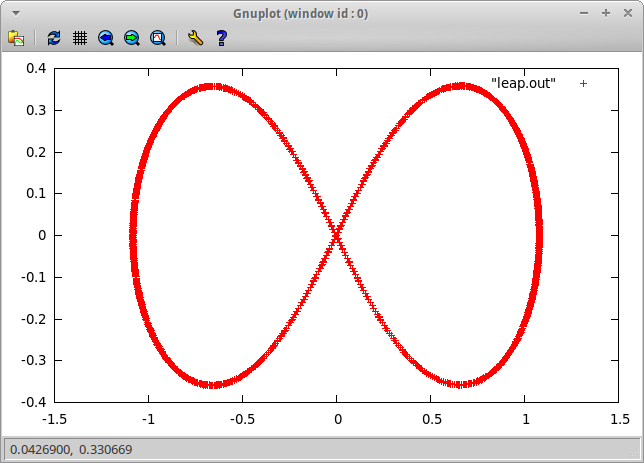
\includegraphics[width=0.75\textwidth]{graphics/gnuplot.png}
  \caption{Execution example}
\end{figure}

